\section{Results}

See comments in source

\begin{figure}[h]
\centering
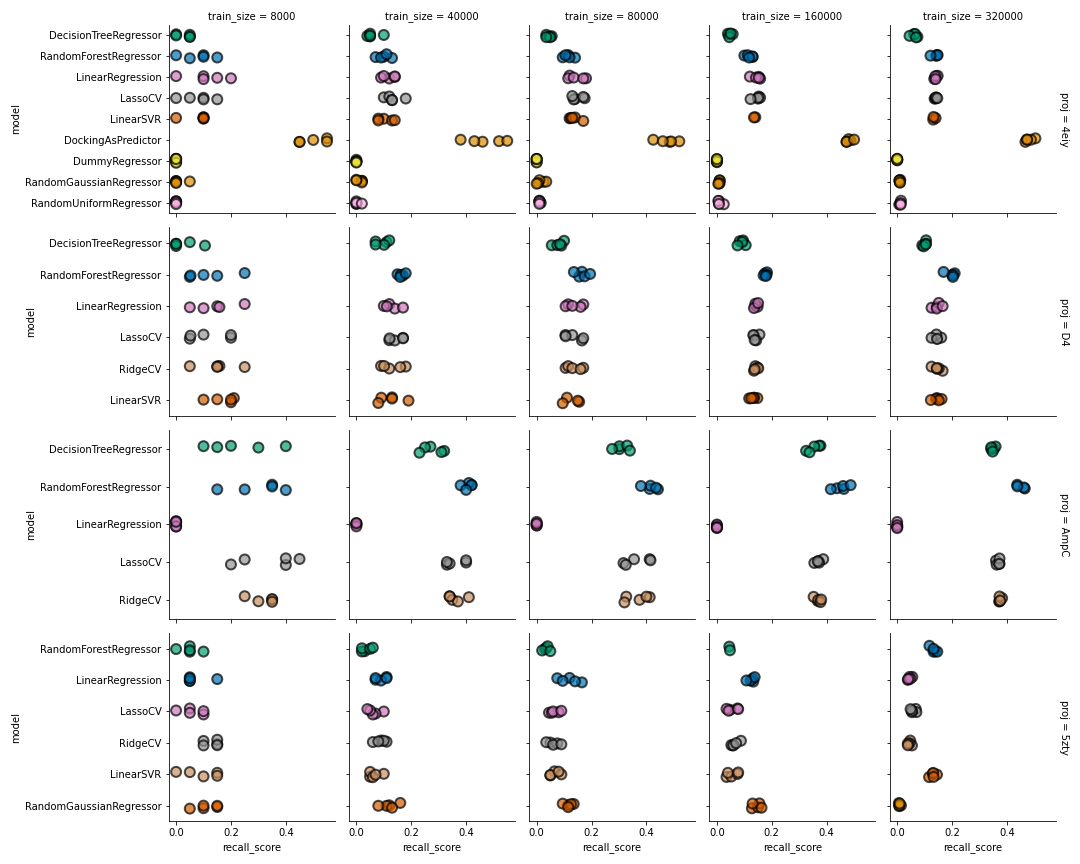
\includegraphics[width=0.8\textwidth]{figures/Figure_4.png}
\caption{Figure 4: Model performance versus training and inference time (in logarithmic scale)}
\end{figure}

% How did we come up with linear models:
% 	- compare performance of all models by "recall"
% 	- compare time with the actual docking time
% 	- test effects of normalization

% Fig 4: selection of the best single model
% 	- A: model performances
% 	- B: model timing
% 	- C: time vs performance distribution + actual docking time cutoff


% How did we come up with iterations scheme:
% 	- compared different train sizes
% 	- compared different regimes (add/noadd)
% 	- compared different ensembling methods
% 	- compare with "docking-as-predictor"

% Fig 5: fine-tuning metaparameters of "iterations" 
% 	- batch size effect on the iterations performance
% 	- add/noadd & different ranking schemes effect
% 	- comparison  of the best model with with docking-as-predictor
% 	- TODO: comparison with the really best single model
